\section{Общие понятия}\label{sec-series-01}

\begin{definition}[Функциональный ряд]\label{def-functional-series}

Для функций \(u_n:\Omega\to\mathbb R\) или \(\mathbb C\) выражение \(\sum_{n=1}^\infty u_n(x)\) называется функциональным рядом. Его частичные суммы: \[
S_n(x)=\sum_{k=1}^n u_k(x).
\] Множество \(E\) точек, в которых числовой ряд сходится, называется множеством поточечной сходимости; сумма ряда на нём обозначается \(S(x)\).

\end{definition}

\begin{definition}[Равномерная сходимость ряда]\label{def-uniform-series}

Ряд \(\sum u_n(x)\) равномерно сходится на \(\Omega\) к \(S\), если \(S_n\rightrightarrows S\) на \(\Omega\). В таком случае \(\Omega\subseteq E\).

Для сходящегося ряда остаток после \(m\) членов равен

\begin{equation}
r_m(x)=S(x)-S_m(x)=\sum_{n=m+1}^\infty u_n(x).
\label{eq-series-remainder}
\end{equation}

\end{definition}

\begin{theorem}[Необходимое условие равномерной сходимости]\label{thm-series-necessary}

Если \(\sum u_n(x)\) равномерно сходится на \(\Omega\), то \(u_n\rightrightarrows0\) на \(\Omega\), то есть \(\lVert u_n\rVert_\infty\to0\).

\end{theorem}

\begin{proof}

Для \(n\ge2\) имеем \(u_n=S_n-S_{n-1}\). Поэтому \[
\lVert u_n\rVert_\infty\le\lVert S_n-S\rVert_\infty+\lVert S_{n-1}-S\rVert_\infty\longrightarrow0.
\]

\end{proof}

\subsection{Два примера}\label{sec-series-01-1}

\begin{example}[Геометрический ряд]\label{exm-geometric-series}

Ряд \(\sum_{n=1}^\infty x^n\) сходится поточечно на \(E=(-1,1)\). На всём \(E\) он не сходится равномерно: \(\sup_{x\in(-1,1)}|x^n|=1\), и необходимое условие не выполнено.

На \(\Omega=[-q,q]\), \(0<q<1\), имеем \[
S_n(x)=\frac{x-x^{n+1}}{1-x},\qquad S(x)=\frac{x}{1-x},
\] \[
\lVert S_n-S\rVert_\infty
=\sup_{|x|\le q}\frac{|x|^{n+1}}{|1-x|}
\le\frac{q^{n+1}}{1-q}\longrightarrow0.
\] Таким образом, ряд равномерно сходится на каждом \([-q,q]\).

\end{example}

\begin{example}[Члены стремятся к нулю равномерно, ряд --- нет]\label{exm-telescoping-series}

На \([0,1]\) рассмотрим \[
\sum_{n=0}^\infty(x^n-x^{n+1})=\sum_{n=0}^\infty x^n(1-x).
\] Для \(n\ge1\) производная члена равна \[
\bigl(x^n(1-x)\bigr)'=x^{n-1}\bigl(n-(n+1)x\bigr).
\] Максимум достигается при \(x=n/(n+1)\), и \[
\sup_{x\in[0,1]}x^n(1-x)
=\left(\frac{n}{n+1}\right)^n\frac1{n+1}\longrightarrow0,
\] так как первый множитель стремится к \(1/e\), а второй --- к нулю.

\begin{center}
\begin{minipage}{\linewidth}
\centering
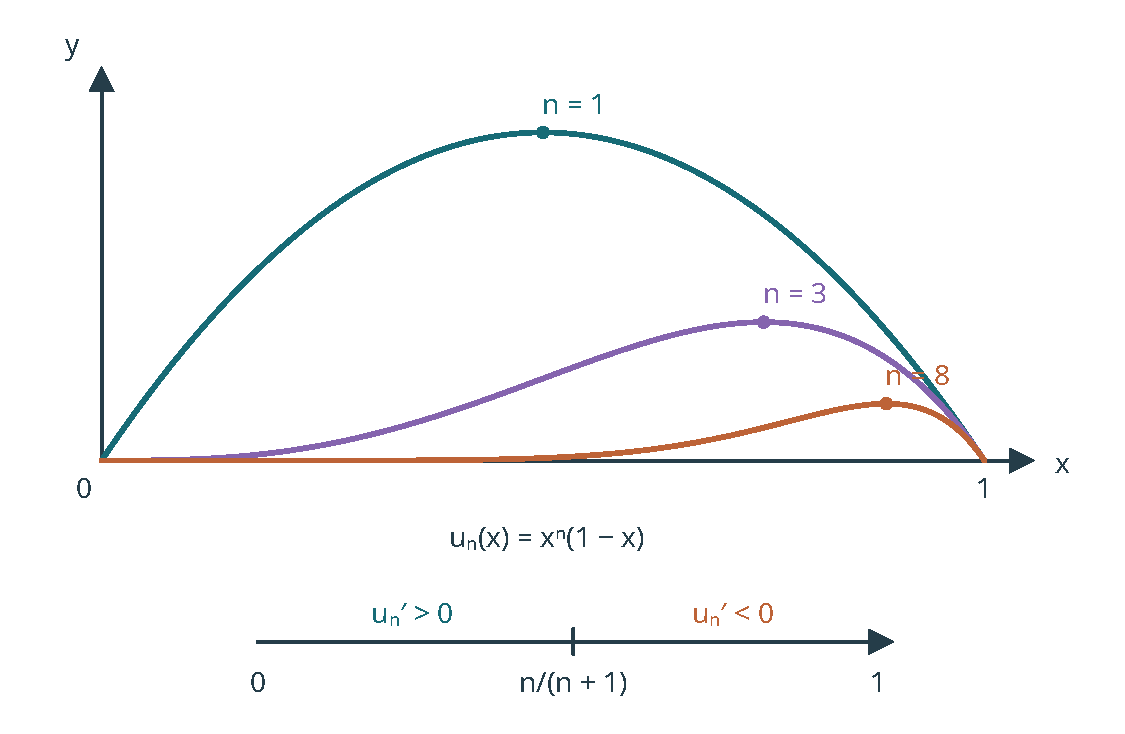
\includegraphics[width=0.85\linewidth]{figures/telescoping.pdf}
\captionof{figure}{Графики членов телескопического ряда и знак производной; максимум при x = n/(n + 1).}\label{fig-telescoping}
\end{minipage}
\end{center}

Однако частичные суммы телескопируются: \[
S_n(x)=\sum_{k=0}^n(x^k-x^{k+1})=1-x^{n+1}\longrightarrow
S(x)=\begin{cases}1,&0\le x<1,\\0,&x=1.\end{cases}
\] Сумма разрывна, хотя все частичные суммы непрерывны. Значит, равномерной сходимости нет. Более того, \(\lVert S_n-S\rVert_\infty=1\).

\end{example}
